\documentclass{standalone}

\usepackage{tikz}

\usetikzlibrary{intersections}

\begin{document}
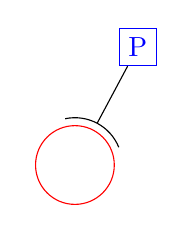
\begin{tikzpicture}
  \coordinate (Origin) at (0,0);
  \coordinate (Xaxis) at (1,0);
  % Note: the minimum size is the diameter, so radius = .5cm
  \node [shape=circle,draw,minimum size=1cm,red] (C) {};
  \node at (0.8,1.5) [shape=rectangle,draw,blue] (P) {P};
  \path [name path=P--C] (P) -- (C);
  \path [name path=Rim] (0,0) circle(0.6cm);
  \path [name intersections={of=P--C and Rim}];
  % This stores in \pgfmathresult the angle between \vec{Origin
  % intersection-1} and the x-axis
  \pgfmathanglebetweenpoints{%
    \pgfpointanchor{Origin}{center}}{%
    \pgfpointanchor{intersection-1}{center}}
  \let\myendresult\pgfmathresult
  \path [draw] (intersection-1) arc[start angle=\myendresult,delta
    angle=-40,radius=0.6cm]; 
  \path [draw] (intersection-1) arc[start angle=\myendresult,delta
    angle=40,radius=0.6cm]; 
  \path [draw] (P) -- (intersection-1);
\end{tikzpicture}
\end{document}